\chapter{Chygraphs with meta-complexes}
\label{ch:metacomplex}

Chapter~\ref{ch:gbp}'s repair works by leaving the chygraph: it builds a region
graph beside the network and passes messages on that. There is a second repair
that does not leave it, and it uses a freedom the construction already has ---
a complex may contain complexes. Merge two complexes that share two or more
atoms into one, and the pairwise overlap is gone. Whether that is enough to
make the answer exact is measured in Sec.~\ref{sec:mergeerror}, and it is not
always.

\begin{figure}[t]
\centering
\begin{adjustbox}{max width=\linewidth}
\begin{tikzpicture}
% ---------- left: two complexes with non-trivial overlap
\node[nd] (a0) at (-5.0,0) {};
\node[nd] (a1) at (-4.05,0.6) {};
\node[nd] (a2) at (-4.05,-0.6) {};
\node[nd] (a3) at (-3.1,0) {};
\node[lb,anchor=east] at (-5.12,0) {$0$};
\node[lb,anchor=west] at (-2.98,0) {$3$};
\draw[lnk] (a0)--(a1) (a0)--(a2) (a1)--(a2) (a1)--(a3) (a2)--(a3);
\begin{scope}[on background layer]
  \node[cx,fit=(a0)(a1)(a2)] {};
  \node[cxb,fill opacity=0.72,fit=(a1)(a2)(a3)] {};
\end{scope}
\node[lb,anchor=north,align=center] at (-4.05,-1.4)
  {two complexes sharing\\the pair $\{1,2\}$};

\node[lb] at (-1.9,0) {$\Longrightarrow$};
\node[tb,anchor=south] at (-1.9,0.16) {merge};

% ---------- right: one meta-complex
\node[nd] (b0) at (-0.7,0) {};
\node[nd] (b1) at (0.25,0.6) {};
\node[nd] (b2) at (0.25,-0.6) {};
\node[nd] (b3) at (1.2,0) {};
\draw[lnk] (b0)--(b1) (b0)--(b2) (b1)--(b2) (b1)--(b3) (b2)--(b3);
\begin{scope}[on background layer]
  \node[cxb,fill opacity=0.9,fit=(b0)(b1)(b2)(b3)] (MC) {};
\end{scope}
\node[lb,anchor=north,align=center] at (0.25,-1.4)
  {one complex of four atoms,\\$2^{4}=16$ interior states};

% ---------- inclusion view underneath
\node[cpx] (mc) at (5.5,0.85) {};
\node[cpx] (c1) at (4.8,-0.1) {};
\node[cpx] (c2) at (6.2,-0.1) {};
\node[atm] (x0) at (4.15,-1.05) {};
\node[atm] (x1) at (5.05,-1.05) {};
\node[atm] (x2) at (5.95,-1.05) {};
\node[atm] (x3) at (6.85,-1.05) {};
\draw[lnk] (mc)--(c1) (mc)--(c2);
\draw[lnk] (c1)--(x0) (c1)--(x1) (c1)--(x2);
\draw[lnk] (c2)--(x1) (c2)--(x2) (c2)--(x3);
\node[lb,anchor=west] at (5.68,0.85) {meta-complex};
\node[lb,anchor=north,align=center] at (5.5,-1.4)
  {as an inclusion: a complex\\whose members are complexes};
\end{tikzpicture}
\end{adjustbox}
\caption{\textbf{The meta-complex construction.} Two complexes that share more
than one atom are replaced by the single complex holding the union of their
atoms, whose interior is then summed exactly. Nothing is added to the
formalism to do it: a complex whose members are complexes is what a chygraph
already is (right), the freedom Chapter~\ref{ch:satisfiability} used to nest
clauses, and Eq.~\eqref{eq:emitted} constrains only that the interior can be
enumerated. On this example the overlap is gone because there is nothing left
for it to overlap with, and the whole of Sec.~\ref{sec:cavityfail}'s discrepancy
goes with it. On a family that merges to several meta-complexes it need not:
merging removes pairwise overlap and not every cycle, which is what
Sec.~\ref{sec:mergeerror} measures. What the construction costs is $2^{c}$ on
the largest merged complex.}
\label{fig:metacomplex}
\end{figure}

\section{Merging complexes}
\label{sec:merging}
\index{merging complexes|textbf}
\index{meta-complex|textbf}
\index{incidence structure|textbf}

A more direct repair than a region graph: if two complexes share more than one
atom, stop treating them as two. Merge them into a single \emph{meta-complex} holding the
union of their atoms, and sum its interior exactly.

Nothing is added to the formalism to do this. A complex whose vertices are
complexes is what a chygraph is --- the freedom Chapter~\ref{ch:satisfiability}
used to nest clauses --- and Eq.~\eqref{eq:emitted} constrains only that the
interior can be enumerated, not its size or internal structure. On
Fig.~\ref{fig:sharededge}'s example the merge is immediate: the two triangles
become one complex of four atoms, its $2^{4}=16$ interior states are summed
exactly, and no overlap remains. Section~\ref{sec:twotriangles}'s discrepancy
disappears, by a route that needs no region graph and no parent-to-child
update.

So the repair removes the obstruction the part is named for. Whether that makes
it \emph{exact} is a second question, and the answer is no in general
(Sec.~\ref{sec:mergeerror}).

\paragraph{Merging is a percolation problem.} The cost is $2^{c}$ on the merged
complex, so the question is how large the merging grows.

Put a node on every complex, and a link between two complexes that share two or
more atoms. The meta-complexes are the connected components of that graph. The
repair is affordable exactly while that graph has \emph{no giant component} ---
and the moment it has one, the merging swallows a finite fraction of the network
into a single complex whose interior cannot be enumerated at any price.

Two details make the closure slightly more than one pass of connected
components. Merging is iterated: two meta-complexes assembled from disjoint
components can still share two atoms between their \emph{unions}, so the
procedure must be run to a fixed point. And the merged complex inherits every
inclusion of its parts, so its chy-degree is the sum --- which is what makes the
component grow.

\section{Non-trivial overlap loops}
\label{sec:mergeerror}

Merging removes every \emph{pairwise} violation by construction: run to a fixed
point, no two surviving complexes share more than one atom. That is the
condition Sec.~\ref{sec:treelike} states, and it is tempting to stop there and
call the result exact. It is not sufficient, and the reason is the one this part
opened with, one level higher again.

Pairwise intersections of at most one node do not make the incidence structure a
tree. Three or more complexes can meet in as many different single nodes and
close a cycle complex--node--complex--node--complex--node, and the chygraph
recursion is a Bethe calculation on that structure. Where such a cycle survives
the merge, so does an error.

The smallest example needs no merging at all, and is worth seeing before the
measurement (Fig.~\ref{fig:ring}). Glue $k$ triangles in a ring, each meeting
the next at one vertex. Every pair of complexes shares exactly one node, so the
condition of Sec.~\ref{sec:treelike} is satisfied --- and the incidence
structure is a ring of $2k$ steps, not a forest.

\begin{figure}[t]
\centering
\begin{adjustbox}{max width=\linewidth}
\begin{tikzpicture}[scale=1.0]
% four triangles glued in a ring at single vertices.  The complexes are drawn as
% filled triangles rather than fitted boxes: axis-aligned boxes round a ring
% overlap into one square and hide the very structure the figure is about.
\def\R{1.75}
\foreach \i in {0,1,2,3}{
  \pgfmathsetmacro{\ang}{90*\i}
  \node[nd] (h\i) at ({\R*cos(\ang)},{\R*sin(\ang)}) {};
  \pgfmathsetmacro{\anga}{90*\i+45}
  \node[nd] (t\i) at ({1.70*\R*cos(\anga)},{1.70*\R*sin(\anga)}) {};
}
\begin{scope}[on background layer]
  \foreach \i/\j in {0/1,1/2,2/3,3/0}{
    \fill[black!8,draw=black!40,line width=7pt,line join=round]
      (h\i.center)--(t\i.center)--(h\j.center)--cycle;
  }
\end{scope}
\foreach \i/\j in {0/1,1/2,2/3,3/0}{
  \draw[lnk] (h\i)--(h\j) (h\i)--(t\i) (t\i)--(h\j);
}
\foreach \i in {0,1,2,3}{
  \pgfmathsetmacro{\anga}{90*\i+45}
  \node[lb,black!55] at ({1.16*\R*cos(\anga)},{1.16*\R*sin(\anga)})
    {$A_{\i}$};
}
\node[lb,anchor=north,align=center] at (0,-3.35)
  {four complexes, every pair\\meeting in at most one node};

% the incidence structure beside it
\begin{scope}[xshift=6.4cm]
  \foreach \i in {0,1,2,3}{
    \pgfmathsetmacro{\ang}{90*\i+45}
    \node[cpx] (c\i) at ({1.15*cos(\ang)},{1.15*sin(\ang)}) {};
    \pgfmathsetmacro{\angh}{90*\i}
    \node[atm] (a\i) at ({1.15*cos(\angh)},{1.15*sin(\angh)}) {};
  }
  \draw[lnk,line width=1.0pt] (c0)--(a1) (a1)--(c1) (c1)--(a2) (a2)--(c2)
                              (c2)--(a3) (a3)--(c3) (c3)--(a0) (a0)--(c0);
  \node[lb,anchor=north,align=center] at (0,-3.35)
    {the incidence structure: a cycle\\of eight steps, not a forest};
\end{scope}
\end{tikzpicture}
\end{adjustbox}
\caption{\textbf{The pairwise condition is not sufficient.} Left: four triangles
glued in a ring, each meeting the next at a single vertex. No two complexes
share two atoms, so Sec.~\ref{sec:treelike}'s test passes. Right: the atom
--complex incidence structure of the same object, which is a cycle. The loop
was never absorbed into any complex; it runs between them, and merging cannot
reach it because merging removes only a loop that lies inside a shared
\emph{pair} of atoms. Table~\ref{tab:ring} is what the recursion then does.}
\label{fig:ring}
\end{figure}

\begin{table}[t]
\centering\small
\begin{tabular}{rrccrr}
\hline\hline
$k$ & $n$ & pairwise test & incidence a forest &
  $\beta J=0.3$ & $\beta J=0.8$\\
\hline
$4$ & $8$ & passes & no & $-0.0180$ & $-0.4277$\\
$5$ & $10$ & passes & no & $-0.0066$ & $-0.3758$\\
$6$ & $12$ & passes & no & $-0.0024$ & $-0.3292$\\
$8$ & $16$ & passes & no & $-0.0003$ & $-0.2506$\\
\hline\hline
\end{tabular}
\caption{\textbf{Error of the cavity method on a ring of $k$ triangles.} Each
satisfies Sec.~\ref{sec:treelike}'s condition exactly and none is exact. The
error falls as the ring lengthens, which is what makes this a short-loop effect
rather than a defect of the scheme: the correlation that has to travel the whole
way round weakens with the distance. Computed in
\code{figs/overlap.py:check\_ring}.}
\label{tab:ring}
\end{table}

Table~\ref{tab:mergeerr} measures the same thing on the merged families of the
three classes.

\begin{table}[t]
\centering\small
\begin{tabular}{lrrrl}
\hline\hline
class & runs & acyclic & exact & error in $\ln Z$\\
\hline
hyperbolic & $60$ & $60$ & $60$ & $<10^{-12}$\\
Karrer--Newman & $60$ & $20$ & $20$ & up to $2.25$\\
real & $120$ & $120$ & $120$ & $<10^{-12}$\\
\hline\hline
\end{tabular}
\caption{\textbf{Error of the chygraph built from meta-complexes.} All $240$
merged families are treelike --- no two complexes share more than one atom ---
but only $200$ have an acyclic incidence structure, and exactness follows the
second condition and not the first. Every acyclic run is exact to
$3\times10^{-13}$; every cyclic run is not, by between $5\times10^{-3}$ and
$2.25$, median $0.18$. Generated by \code{probe/merge\_lnz.py}.}
\label{tab:mergeerr}
\end{table}

\begin{figure}[t]
\centering
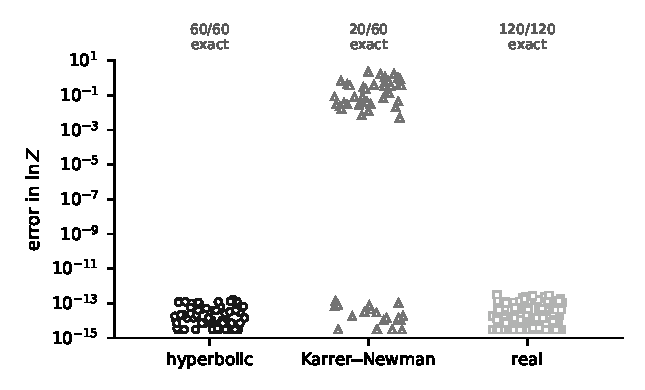
\includegraphics[width=\linewidth]{figs/fig-merge-error.pdf}
\caption{\textbf{Error in $\ln Z$.} For the $240$ runs, one column per class. Hyperbolic random graphs and real
neighbourhoods come out exact throughout, at machine precision. The placed
ensemble carries an error on two thirds of its runs, between $5\times10^{-3}$
and $2.25$ in $\ln Z$. The class is the comparison, which is why it is the axis;
what within the class decides the outcome is Fig.~\ref{fig:coretransition}.
Generated by \code{figs/overlap.py} from
\code{probe/merge\_lnz.py}.}
\label{fig:mergeerror}
\end{figure}

\begin{figure}[t]
\centering
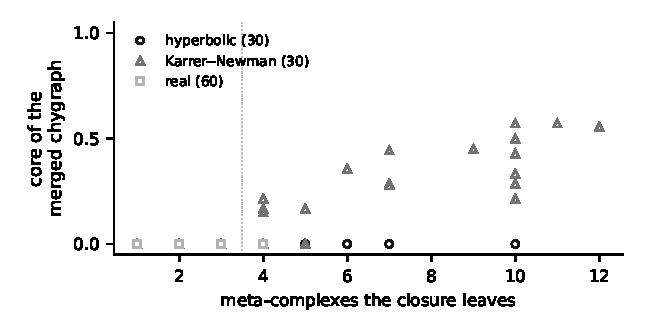
\includegraphics[width=\linewidth]{figs/fig-core-meta.pdf}
\caption{\textbf{Fraction of nodes in the core.} Core fraction
$P_{C}(\mathrm{Ising},\mathrm{BP}_{\chi_{m}})$ of the merged chygraph, by class --- the quantity of
Fig.~\ref{fig:corebonds} evaluated on the closure rather than on the cliques. Merging drives it
to zero on $100$ of the $120$ instances: every hyperbolic and every real one,
and a third of the placed ones, which are exactly the instances the recursion
then solves exactly. Where a core survives it runs between $0.15$ and $0.57$ of
the atoms, and so does the error. Computed by
\code{probe/core\_fraction.py}.}
\label{fig:coremeta}
\end{figure}

\begin{figure}[t]
\centering
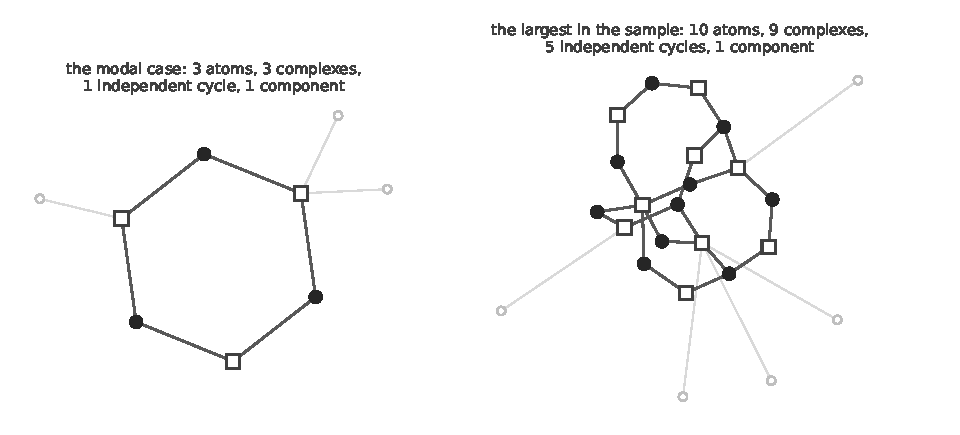
\includegraphics[width=\linewidth]{figs/fig-core-example.pdf}
\caption{\textbf{What the messages are left with.} The surviving core of two
Karrer--Newman instances, drawn as inclusions in the vocabulary of
Sec.~\ref{sec:drawing}: filled circles are atoms, open squares complexes, a
line is membership. Faint atoms are those leaf removal stripped, shown to make
clear what went. Left, the modal case, eight of the twenty: three complexes
meeting pairwise at one atom each, a six-step ring, which is
Fig.~\ref{fig:ring} at $k=3$ found in the data rather than constructed. Right,
the largest in the sample: ten atoms across nine complexes carrying five
independent cycles. Both are a \emph{single} connected cluster, and so is every
other one --- the residue is never a scattering of separate pieces. Generated by
\code{figs/overlap.py} from \code{probe/core\_fraction.py}.}
\label{fig:coreexample}
\end{figure}

Figure~\ref{fig:coremeta} says the same thing as a quantity rather than a test.
Before merging, not one of the $120$ instances is core-free: propagation on the
clique chygraph is left with between a half and three quarters of the atoms it
cannot resolve (Fig.~\ref{fig:corebonds}). After merging the core is gone on
$100$ of them --- every hyperbolic instance, every real one, a third of the
placed ones --- and those hundred are precisely the hundred the recursion solves
exactly. A core of zero and an acyclic incidence structure are the same
statement, one counted and one tested, and either can be read off before the
messages are run.

What survives on the twenty placed instances that keep a core is small, and it
is one thing rather than many (Fig.~\ref{fig:coreexample}). Every one of the
twenty is left with a \emph{single} connected cluster --- a median of four
complexes and four or five atoms, never more than ten across nine --- and none
is left with two. That is structural rather than lucky: the closure has
already absorbed every pair of complexes sharing two atoms, so whatever survives is joined at
single atoms, and a single atom joining two otherwise separate pieces is a cut
vertex, which leaf removal strips. Anything that would have separated the
residue has been removed by the time the residue exists.

Half of the twenty carry one independent cycle, and eight of those are the
minimal ring of Fig.~\ref{fig:ring} with $k=3$: three complexes, three atoms,
six steps. The other half carry two to five interlocking cycles in one tangle.
So the obstruction is not diffuse damage spread over the instance. It is one small
knot, and the whole of the error in $\ln Z$ comes from it.

The correspondence is exact and it goes both ways. All $200$ runs whose merged
incidence structure is acyclic come out exact, to $3\times10^{-13}$ at worst.
All $40$ that retain a cycle come out wrong, by $5\times10^{-3}$ to $2.25$ in
$\ln Z$ with a median of $0.18$. Not one instance falls on the wrong side. The
condition for the meta-complex chygraph to be exact is that the merged incidence
structure is a forest, and merging to a treelike family does not deliver it.

The classes divide sharply. On hyperbolic random graphs and on real
neighbourhoods the merge closure is exact everywhere --- largely because it has
swallowed the instance whole, and a single complex has no
incidence structure left to close a cycle in. On the Karrer--Newman ensemble
only a third of the merged families are acyclic, and the other two thirds keep
an error.

That is not merging failing where the plain calculation would have done better.
Merging is a generalisation of it --- with nothing to merge the two coincide ---
and on these instances it takes the median error from $0.289$ to $0.033$. It
improves the answer by a factor of ten and stops short of exactness, because the
loops it leaves are the ones of Fig.~\ref{fig:ring}: running between complexes
rather than inside a shared pair of atoms, where merging has no purchase. The
ensemble on which the closure is cheap is the ensemble on which it leaves those
loops, and for one reason --- it leaves many small meta-complexes rather than
one large one, and many small complexes are what closes a cycle.

A cycle needs at least three complexes meeting in at least three distinct single
atoms, so a closure leaving three meta-complexes or fewer cannot have one, and in
the whole sample none does. What decides exactness is therefore not how large
the largest meta-complex is but how \emph{many} the closure leaves. The two run in opposite directions, and a
closure cheap enough to enumerate is for that reason the more likely to have
left a cycle behind. Section~\ref{sec:coretransition} asks what in the ensemble
decides how many there are.

\section{Core percolation transition of non-trivial overlap}
\label{sec:coretransition}
\index{incidence branching|textbf}
\index{core percolation}
\index{Erd\H{o}s--R\'enyi 2-core}

Everything measured so far is an outcome. How many meta-complexes the closure
leaves, how much core $P_{C}(\mathrm{Ising},\mathrm{BP}_{\chi_{m}})$ survives, how large the error is --- these are things read
off an instance after the fact, and none of them says what \emph{produces} the
cycles. The placed ensemble is the one class here with control parameters one
can turn: $n$, the single edges per vertex $s$, and the triangles per vertex
$t$. Turning them locates a threshold.

\paragraph{The branching ratio.} Follow an atom into a complex and out through
the complex's other atoms. A complex of cardinality $c$ offers $c-1$ ways on, so
an atom carrying $s$ edge memberships and $t$ triangle memberships branches
\begin{equation}
  b=s\cdot 1+t\cdot 2
  \label{eq:branching}
\end{equation}
ways at the next step. A branching process survives when its ratio exceeds one,
and the 2-core of the incidence structure is what survives, so the core should
appear at $b=1$ and not before --- whatever mixture of edges and triangles
supplies it. None of that is new: it is the $k$-core transition of
\citet{pittel1996} at $k=2$, equivalently the point at which
\citeauthor{bauer2001}'s standard leaf removal stops consuming the graph
\citep{bauer2001}, and it is where the loops that defeat belief propagation
appear \citep{mezard2009}. At $t=0$ the
complexes are bare edges, the chygraph is a graph, and
Eq.~\eqref{eq:branching} says $s=1$: the Erd\H{o}s--R\'enyi $2$-core at mean
degree one, which fixes the scale independently. What is measured here is not
the transition but where a chygraph ensemble sits relative to it.

\begin{figure}[t]
\centering
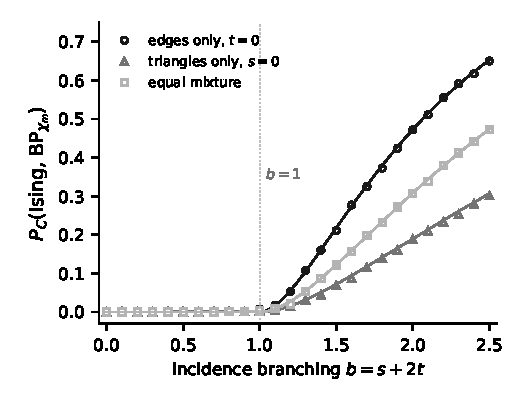
\includegraphics[width=\linewidth]{figs/fig-core-transition.pdf}
\caption{\textbf{Phase transition in the Karrer--Newman ensemble.} Core
fraction $P_{C}(\mathrm{Ising},\mathrm{BP}_{\chi_{m}})$, triangles only in the
right panel, against the branching ratio of
Eq.~\eqref{eq:branching}. Left: three lines through the $(s,t)$ plane at
$n=1600$ --- edges only, triangles only, and an equal mixture. All three are
core-free below $b=1$ and rise continuously above it, so the threshold depends
on $s$ and $t$ only through $b$ while the amplitude above it does not. Right:
the triangles-only line at four sizes, with standard errors over $24$
realisations. The two largest agree within them --- $0.0870$ against $0.0863$ at
$b=1.6$ --- while $n=200$ sits below, so the curves converge from below with $n$
rather than coinciding at every size. Generated by
\code{figs/overlap.py} from \code{probe/karrer\_core\_sweep.py}.}
\label{fig:coretransition}
\end{figure}

That is what the sweep finds. Below $b=1$ every family is core-free to within
$1.5\times10^{-3}$ at $n=1600$; above it the core grows continuously from zero,
reaching $0.28$, $0.16$ and $0.09$ at $b=1.6$ on the three lines. The rise is
continuous rather than a jump, which makes it a second-order transition in the
usual sense.

The finite-size evidence, stated exactly, since Table~\ref{tab:knfinite} shows
this part is not immune to reading a crossover as a transition. Below the
threshold the core \emph{falls} with $n$, from $0.0067$
at $n=200$ to $0.0030$ at $n=1600$ at $b=1$, as it must if it is heading for
zero. Above it the core rises with $n$ but converges: at $b=1.6$ the steps are
$+0.007$, $+0.012$ and $+0.0007$ across the four sizes, so $n=800$ and $n=1600$
agree to well within their standard errors of about $0.004$. The two sides of
$b=1$ move in opposite directions with $n$ and both have settled by $n=800$,
which is what a transition looks like and a crossover does not.

Two things follow that the outcome plots could not give.

The threshold collapses onto $b$ and the amplitude does not. At $b=1.6$ the
edges-only line carries three times the core of the triangles-only line, because
a triangle absorbs two of its atoms' branchings into one interior while two
edges spend them on two complexes. So the ensemble's parameters decide
\emph{whether} there is a core through $b$ alone, and decide \emph{how much}
through the cardinality as well.

And it explains why Sec.~\ref{sec:mergeerror}'s instances behave as they do. The
placed ensemble was sampled at $s=1$ or $1.5$ and $t=1$ to $3$, so $b$ between
$3.5$ and $7$ --- far above threshold, which is why two thirds of those
instances keep a core. It is not that the placed ensemble is peculiar. It is that it was
measured deep in the phase where cores exist, and the same would be true of any
ensemble put there.

\section{Conclusions}
\label{sec:part4-conclusions}

\paragraph{On real networks the repair works.} Chapter~\ref{ch:overlap}
measured the cavity method erring by a median of $5.06$ in $\ln Z$ on the $120$
real neighbourhoods --- a factor of $150$ in $Z$ --- because their complexes
share more than one atom. Merging those complexes and solving the resulting
chygraph removes the error entirely: all $120$ come out exact, the worst
discrepancy being $3\times10^{-13}$, which is the arithmetic and not the
approximation. The same holds on all $60$ hyperbolic instances. The construction
does not leave the formalism: a merged complex is a complex, and a merged
chygraph is a chygraph.

\paragraph{The condition it meets.} The chygraph recursion is exact when the
incidence structure of its complexes is a forest.
Merging does not guarantee that --- it removes pairwise overlap, and three
complexes can still close a cycle through three single atoms, as
Fig.~\ref{fig:ring} shows with four triangles that pass Sec.~\ref{sec:treelike}'s
test and are still wrong. But on real neighbourhoods it delivers a forest every
time, because the closure there merges nearly everything into one to three large
complexes and a large complex absorbs the loops into an interior that is summed
exactly. Over all $240$ runs the criterion is exact in both directions: every one
of the $200$ acyclic families is exact, every one of the $40$ cyclic ones is
not, by $5\times10^{-3}$ to $2.25$ in $\ln Z$. Nothing falls on the wrong side.

\paragraph{Where the cycles come from.} All $40$ cyclic families are
Karrer--Newman, and Sec.~\ref{sec:coretransition} locates the cause in the
ensemble's parameters. Following an
atom into a complex of cardinality $c$ and out through its $c-1$ other atoms
gives an incidence branching $b=s+2t$; the 2-core of that structure is what a
branching process at ratio $b$ leaves behind, so it should appear at $b=1$
whatever mixture of edges and triangles supplies it, and it does. Below the
threshold every family is core-free and the core falls with $n$; above it the
core grows continuously from zero and settles by $n=800$. The rise is continuous
rather than a jump, which makes it second-order, and at $t=0$ the statement
reduces to the Erd\H{o}s--R\'enyi $2$-core at mean degree one, which fixes the
scale from outside this book.

The instances of Sec.~\ref{sec:mergeerror} were drawn at $b$ between $3.5$ and
$7$, far above threshold, so two thirds of them keeping a core follows from
where they were sampled rather than from the ensemble. The hyperbolic and real
neighbourhoods, whose closures leave one to three complexes, are on the other
side of it.

\paragraph{What remains open.} All of this is instance-level. It takes an
explicit list of complexes and an explicit interaction, where every other
calculation in the book carries a message per chy-degree class. The ensemble
version --- a message indexed by region type, over a region graph that is itself
a random object --- is not supplied here, and Chapter~\ref{ch:outlook} lists it
with the other things this book does not do. Section~\ref{sec:coretransition} is
the one place in the part where an ensemble question is answered in the
ensemble's own terms, and it answers a question about the structure rather than
about the messages.


\section{Checks}
\label{sec:merge-checks}

\checkhead{Known results}
That a complex may contain complexes is the definition of
Chapter~\ref{ch:chygraphs}, not a new construction, and Eq.~\eqref{eq:emitted}
applies to a meta-complex unchanged. The Karrer--Newman ensemble is
\citeauthor{karrer2010}'s. The branching threshold of
Sec.~\ref{sec:coretransition} has an anchor outside this book: at $t=0$ the
complexes are bare edges, the chygraph is a graph, and $b=1$ is the
Erd\H{o}s--R\'enyi $2$-core at mean degree one, which the sweep reproduces.

\checkhead{New results}
The error the merge closure leaves, and where the core that carries it appears,
are new. The closure is iterated to a fixed point rather than run once, because
two meta-complexes assembled from disjoint components can still share two atoms
between their unions. Exactness is tested against enumeration on every instance,
and the acyclicity of the merged incidence structure is tested directly rather
than inferred from the pairwise condition; the two disagree on $40$ of $240$
runs, which is the point of Sec.~\ref{sec:mergeerror}. Both the failure of
Chapter~\ref{ch:overlap} and the repair here are computed by one routine,
\code{ChygraphBP}, so the two sets of numbers differ in the complex family and
in nothing else.

\checkhead{Partial results}
The transition is measured on the Karrer--Newman ensemble alone, because it is
the only one of the three classes with parameters that can be turned: a
hyperbolic random graph is set by $\tau$ and $\ave{k}$, and a real network is
whatever it is. That the threshold sits at $b=1$ for any mixture is argued from
the branching ratio and checked on three lines through the $(s,t)$ plane, not
proved here; for $c=2$ it is \citeauthor{pittel1996}'s result, and the $b=1$
anchor is \citeauthor{bauer2001}'s $\alpha=1$, the companion of the $\ave{k}=e$
that Chapter~\ref{ch:cover} uses. The finite-size evidence is stated rather than assumed --- the core
falls with $n$ below the threshold and rises to a limit above it, settling by
$n=800$ --- because Table~\ref{tab:knfinite} shows this part is not immune to
reading a crossover as a transition. And the whole chapter is instance-level:
the ensemble version is not supplied here, and Chapter~\ref{ch:outlook} lists it
with the other things this book does not do.
